\newcommand{\blueSection}[1]{%
	\vspace{0.5cm}
	\phantomsection
	\addcontentsline{toc}{section}{#1}
	{\Large \bfseries \color{blue!80!black} #1}
	\vspace{2mm}
	{\color{blue!80!black}\hrule height 1pt}
	\vspace{0.3cm}
}

\blueSection{Objective}
\begin{itemize}
	\item To construct and configure a functional full-wave bridge rectifier circuit on a breadboard using four semiconductor diodes.
	\item To investigate the detailed cycle-by-cycle conduction dynamics of the bridge topology during both alternating polarity cycles.
	\item To capture, visualize, and compare the input and rectified voltage waveforms utilizing a Digital Storage Oscilloscope (DSO).
	\item To evaluate critical operational metrics, including average DC output voltage ($V_{DC}$), RMS voltage ($V_{rms}$), ripple factor ($r$), and rectification efficiency ($\eta$).
	\item To examine the filtering behavior of a parallel reservoir capacitor on voltage stabilization and evaluate experimental performance against theoretical derivations.
\end{itemize}

\blueSection{Introduction}
Modern electronic instrumentation predominantly demands a reliable DC supply for consistent operation, whereas municipal power distribution relies almost exclusively on alternating current (AC). Rectification serves as the core process to reconcile this difference by converting bidirectional AC inputs into unidirectional pulsating DC signals. Among various configurations, the full-wave bridge rectifier is widely utilized due to its superior transformer utilization factor and elimination of center-tapped transformer requirements. Utilizing four diodes configured in a closed bridge topology, the circuit ensures continuous current delivery through the load in a single direction regardless of source polarity. As the raw rectified output inherently exhibits significant ripple components, smooth DC delivery is subsequently achieved through parallel capacitive filtering.

\blueSection{Theory}

\subsection{Cycle-by-Cycle Conduction Analysis}
Consider an AC voltage source supplying the bridge arrangement defined as:
\[
v_s(t) = V_m \sin(\omega t),
\]
where $V_m = V_{rms}\sqrt{2}$ denotes peak secondary voltage and $\omega = 2\pi f$ is the angular frequency of the input.
\begin{itemize}
	\item \textbf{Positive Half-Cycle ($0 < \omega t < \pi$):} The upper terminal maintains a positive potential relative to the lower terminal. Diodes $D_1$ and $D_4$ become forward-biased and conduct, while $D_2$ and $D_3$ remain reverse-biased (off). Current flows from the source through $D_1$, passes downward across load $R_L$, and completes its path via $D_4$.
	\item \textbf{Negative Half-Cycle ($\pi < \omega t < 2\pi$):} Upon polarity reversal, diodes $D_2$ and $D_3$ transition to forward conduction, while $D_1$ and $D_4$ block. The current trajectory across $R_L$ remains identically directed from top to bottom, routed through $D_2$ and $D_3$.
\end{itemize}
Consequently, current traverses the load during both half-cycles in an identical direction, yielding an output ripple frequency twice that of the input source ($f_{\text{out}} = 2 f_{\text{in}}$).

\subsection{Mathematical Formulation of Rectifier Parameters}
Accounting for the simultaneous conduction of two series diodes with combined forward drops ($V_D \approx \qty{0.7}{\volt}$ each), the peak output voltage ($V_{mo}$) is governed by:
\[
V_{mo} = V_m - 2V_D.
\]
The average DC output voltage and RMS output voltage are respectively expressed as:
\[
V_{DC} = \frac{2V_{mo}}{\pi}, \qquad V_{rms} = \frac{V_{mo}}{\sqrt{2}}.
\]
The ripple factor ($r$), reflecting the residual AC component relative to the DC base value, is derived as:
\[
r = \sqrt{\left(\frac{V_{rms}}{V_{DC}}\right)^2 - 1} = \sqrt{\left(\frac{\pi}{2\sqrt{2}}\right)^2-1} \approx 0.482.
\]
This factor remains independent of load resistance and voltage scale. Key performance parameters also include conversion efficiency ($\eta$) and the Peak Inverse Voltage (PIV) rating per diode:
\[
\eta = \frac{P_{DC}}{P_{AC}}\times100\%, \qquad \eta_{\max} = \frac{8}{\pi^2}\approx81.2\%, \qquad \text{PIV} = V_m.
\]

\subsection{Effect of a Capacitive Filter}
Connecting a smoothing capacitor $C$ in parallel with $R_L$ stabilizes the output voltage. The capacitor rapidly charges near peak input ($V_{mo}$) and slowly discharges through $R_L$ during signal decay intervals. Assuming a linear discharge model under small ripple conditions, peak-to-peak ripple voltage and ripple factor are expressed by:
\[
V_{r(p\text{-}p)} \approx \frac{I_{DC}}{2fC} = \frac{V_{DC}}{2fR_LC}, \qquad r \approx \frac{1}{4\sqrt{3}\,fR_LC}.
\]
These expressions demonstrate that increasing either load resistance or filter capacitance significantly minimizes output ripple.

\blueSection{Apparatus and Components}
\begin{table}[h!]
	\centering
	\caption{List of Equipment and Components Used}
	\vspace{2mm}
	\resizebox{\textwidth}{!}{%
		\begin{tabular}{llc}
			\toprule
			\textbf{Item Description} & \textbf{Specification / Rating} & \textbf{Quantity} \\
			\midrule
			Function Generator & Sine wave, \qty{50}{\hertz}, measured peak output \qty{6}{\volt} & 1 \\
			Silicon Rectifier Diodes & 1N4007 & 4 \\
			Load Resistor $R_L$ & \qty{965}{\ohm} & 1 \\
			Electrolytic Filter Capacitor $C$ & \qty{47}{\micro\farad} & 1 \\
			Dual-Channel Digital Storage Oscilloscope (DSO) & With $10\times$ probes & 1 \\
			Solderless Breadboard & Standard Tie-Point & 1 \\
			Connecting Wires & Jumper Wires & As required \\
			\bottomrule
		\end{tabular}%
	}
	\label{tab:apparatus6}
\end{table}
\textit{Note: Function generator output voltage was measured directly via DSO display.}

\blueSection{Circuit Diagram}
\begin{figure}[H]
	\centering
	\begin{circuitikz}[american, scale=0.85]
		\draw (-2,0) to[sV, l=$v_s(t)$] (-2,4);
		\node at (-2,-0.6) [below] {Function Generator};
		\draw (-2,4) -- (0,4) -- (0,2);
		\draw (-2,0) -- (-2,-3) -- (6,-3) -- (6,2);
		\coordinate (L) at (0,2);
		\coordinate (R) at (6,2);
		\coordinate (T) at (3,5);
		\coordinate (Bt) at (3,-1);
		\draw (L) to[D, l=$D_1$] (T);
		\draw (R) to[D, l=$D_2$] (T);
		\draw (Bt) to[D, l=$D_3$] (L);
		\draw (Bt) to[D, l=$D_4$] (R);
		\draw (T) to[R, l=$R_L$] (Bt);
		\draw (T) -- (4.5,5) to[C, l=$C$] (4.5,-1) -- (Bt);
		\draw (Bt) node[ground]{};
		\node at (0,2.4) [above left] {AC$_1$};
		\node at (6,2.4) [above right] {AC$_2$};
		\node at (3,5.4) [above] {$+$ (DC Output)};
	\end{circuitikz}
	\caption{Full-wave bridge rectifier schematic depicting source connection, four-diode bridge layout, load resistor $R_L$, and parallel smoothing capacitor $C$.}
	\label{fig:bridgerectifier}
\end{figure}

\blueSection{Experimental Procedure}
\begin{enumerate}
	\item \textbf{Bridge Assembly:} Position four 1N4007 semiconductor diodes on the breadboard following the bridge orientation in Figure~\ref{fig:bridgerectifier}. Verify anode-cathode alignment systematically.
	\item \textbf{Source Integration:} Connect function generator leads across input terminals $\text{AC}_1$ and $\text{AC}_2$, delivering a \qty{50}{\hertz} sinusoidal wave.
	\item \textbf{Unfiltered Baseline Testing:} Attach load resistor $R_L = \qty{965}{\ohm}$ across output nodes without filtering. Connect DSO Channel 1 to AC input and Channel 2 to load output to measure peak values $V_m$ and $V_{mo}$. Derive parameters $V_{DC}$, $V_{rms}$, ripple factor, and conversion efficiency using theoretical relations.
	\item \textbf{Filtered Analysis:} Connect electrolytic capacitor $C = \qty{47}{\micro\farad}$ across $R_L$ with strict polarity compliance. Observe waveform smoothing on the DSO display and determine filtered DC output and peak-to-peak ripple voltage $V_{r(p\text{-}p)}$.
\end{enumerate}

\blueSection{Theoretical Calculation}
Using measured parameters: $V_m = \qty{6}{\volt}$, diode threshold $V_D = \qty{0.7}{\volt}$, $f = \qty{50}{\hertz}$, and $R_L = \qty{965}{\ohm}$:
\[
V_{mo} = V_m - 2V_D = 6 - 1.4 = \qty{4.60}{\volt},
\]
\[
V_{DC} = \frac{2V_{mo}}{\pi} = \frac{2\times4.60}{3.1416} = \qty{2.928}{\volt}, \qquad
I_{DC} = \frac{V_{DC}}{R_L} = \frac{2.928}{965} = \qty{3.03}{\milli\ampere},
\]
\[
V_{rms(\text{out})} = \frac{V_{mo}}{\sqrt{2}} = \frac{4.60}{1.4142} = \qty{3.253}{\volt},
\]
\[
\eta = \frac{V_{DC}^2/R_L}{V_{rms(\text{out})}^2/R_L}\times100\% = \frac{2.928^2}{3.253^2}\times100\% \approx 81.0\%, \qquad \text{PIV} = V_m = \qty{6}{\volt}.
\]
The theoretical efficiency matches closely with the ideal cap of $\eta_{\max} = 8/\pi^2 \approx 81.2\%$. Incorporating the \qty{47}{\micro\farad} filter capacitor yields:
\[
V_{r(p\text{-}p)} \approx \frac{V_{DC}}{2fR_LC} = \frac{2.928}{2\times50\times965\times47\times10^{-6}} \approx \qty{0.646}{\volt}.
\]

\blueSection{Data Collection}
\label{sec:datacollection6}

\begin{table}[h!]
	\centering
	\caption{Unfiltered Rectifier Performance Parameters}
	\vspace{2mm}
	\resizebox{\textwidth}{!}{%
		\begin{tabular}{ccccccc}
			\toprule
			\textbf{Load $R_L$} & \textbf{Peak Input $V_m$} & \textbf{Peak Output $V_{mo}$} & \textbf{Measured $V_{DC}$} & \textbf{Measured $V_{rms}$} & \textbf{Ripple Factor $r$} & \textbf{Efficiency $\eta$} \\
			\midrule
			\qty{965}{\ohm} & \qty{6}{\volt} & \qty{2}{\volt} & \qty{1.27}{\volt} & \qty{1.41}{\volt} & 0.483 & 81.1\% \\
			\bottomrule
		\end{tabular}%
	}
	\label{tab:unfiltereddata6}
\end{table}

\begin{table}[h!]
	\centering
	\caption{Filtered Rectifier Performance Parameters ($C = \qty{47}{\micro\farad}$)}
	\vspace{2mm}
	\begin{tabular}{cccc}
		\toprule
		\textbf{Load $R_L$} & \textbf{Filter $C$} & \textbf{Measured $V_{DC}$} & \textbf{Ripple $V_{r(p\text{-}p)}$} \\
		\midrule
		\qty{965}{\ohm} & \qty{47}{\micro\farad} & \qty{1.78}{\volt} & \qty{0.44}{\volt} \\
		\bottomrule
	\end{tabular}
	\label{tab:filtereddata6}
\end{table}

\subsection{Oscilloscope Waveforms}
Input and output traces rendered below correspond to captured laboratory measurements.

\begin{figure}[H]
	\centering
	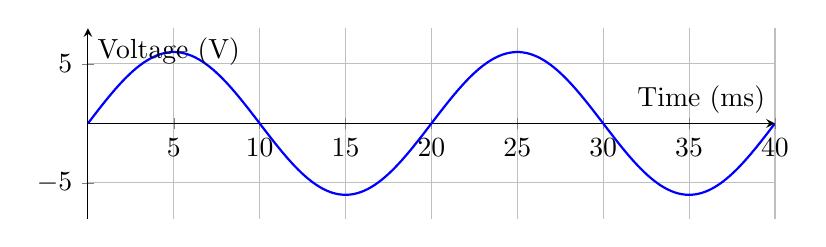
\begin{tikzpicture}
		\begin{axis}[
			width=0.85\textwidth,
			height=4cm,
			xlabel={Time (ms)},
			ylabel={Voltage (V)},
			xmin=0, xmax=40,
			ymin=-8, ymax=8,
			axis lines=middle,
			grid=major,
			]
			\addplot[domain=0:40, samples=200, thick, blue] {6*sin(x/20*360)};
		\end{axis}
	\end{tikzpicture}
	\caption{Sinusoidal input waveform supplied by function generator ($V_m=\qty{6}{\volt}$, $f=\qty{50}{\hertz}$).}
	\label{fig:waveinput6}
\end{figure}

\begin{figure}[H]
	\centering
	\includegraphics[width=0.75\textwidth, keepaspectratio]{waveforms/wave_input_photo}
	\caption{Oscilloscope trace record showing input AC waveform.}
	\label{fig:waveinputphoto6}
\end{figure}

\begin{figure}[H]
	\centering
	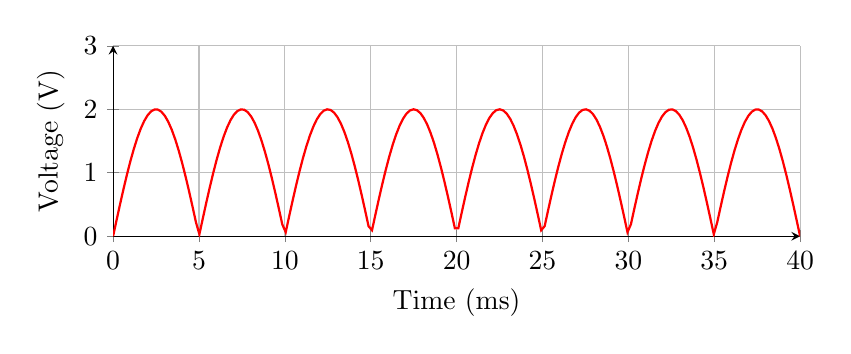
\begin{tikzpicture}
		\begin{axis}[
			width=0.85\textwidth,
			height=4cm,
			xlabel={Time (ms)},
			ylabel={Voltage (V)},
			xmin=0, xmax=40,
			ymin=0, ymax=3,
			axis lines=left,
			grid=major,
			]
			\addplot[domain=0:40, samples=200, thick, red] {2*abs(sin(x/10*360))};
		\end{axis}
	\end{tikzpicture}
	\caption{Unfiltered full-wave rectified output showing periodic pulse frequency doubling ($V_{mo}=\qty{2}{\volt}$).}
	\label{fig:waveoutput6}
\end{figure}

\begin{figure}[H]
	\centering
	\includegraphics[width=0.75\textwidth, keepaspectratio]{waveforms/wave_unfiltered_photo}
	\caption{Oscilloscope trace record of unfiltered full-wave output.}
	\label{fig:waveoutputphoto6}
\end{figure}

\begin{figure}[H]
	\centering
	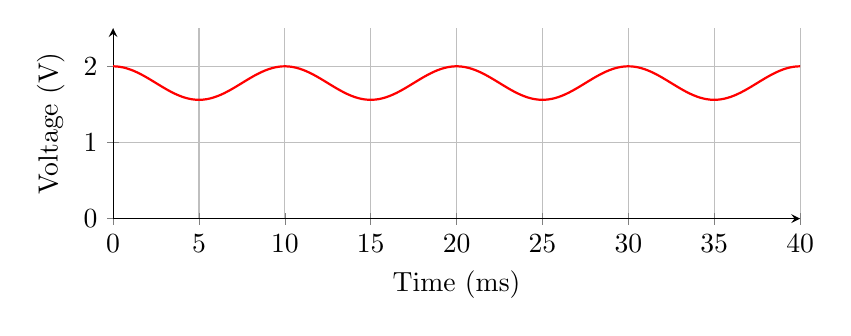
\begin{tikzpicture}
		\begin{axis}[
			width=0.85\textwidth,
			height=4cm,
			xlabel={Time (ms)},
			ylabel={Voltage (V)},
			xmin=0, xmax=40,
			ymin=0, ymax=2.5,
			axis lines=left,
			grid=major,
			]
			\addplot[domain=0:40, samples=200, thick, red] {1.78+0.22*cos(x/10*360)};
		\end{axis}
	\end{tikzpicture}
	\caption{Filtered output profile illustrating smoothing effect around steady DC level ($V_{DC}=\qty{1.78}{\volt}$).}
	\label{fig:wavefiltered6}
\end{figure}

\begin{figure}[H]
	\centering
	\includegraphics[width=0.75\textwidth, keepaspectratio]{waveforms/wave_filtered_photo}
	\caption{Oscilloscope trace record showing capacitor-filtered output.}
	\label{fig:wavefilteredphoto6}
\end{figure}

\blueSection{Result Analysis}
\label{sec:resultanalysis6}
The observed peak output voltage $V_{mo} = \qty{2}{\volt}$ indicates a deviation from the simplified theoretical estimation of \qty{4.60}{\volt}. This discrepancy propagates to derivative variables ($V_{DC}$, $V_{rms}$, $I_{DC}$). Conversely, scale-independent parameters show strong convergence with theoretical benchmarks: the measured ripple factor of $0.483$ matches closely with the theoretical constant of $0.482$, while the conversion efficiency of $81.1\%$ aligns with the $81.2\%$ upper limit. Adding the \qty{47}{\micro\farad} filter capacitor raised the effective DC voltage from \qty{1.27}{\volt} to \qty{1.78}{\volt} while attenuating peak-to-peak ripple to \qty{0.44}{\volt}, confirming successful smoothing.

\blueSection{Conclusion}
The full-wave bridge rectifier circuit was successfully assembled and characterized under a \qty{6}{\volt} peak, \qty{50}{\hertz} input condition. Despite voltage attenuation relative to ideal diode calculations, normalized characteristics including ripple factor and conversion efficiency verified proper full-wave conduction dynamics. Furthermore, integration of capacitive filtering demonstrated significant ripple reduction and DC stabilization, validating the fundamental design principles of power rectification circuits.

\blueSection{References}
\begin{tcolorbox}[colback=gray!5, colframe=gray!40, arc=2mm]
	\begin{enumerate}
		\item Boylestad, R. L., \& Nashelsky, L. (2013). \textit{Electronic Devices and Circuit Theory} (11th ed.). Pearson.
		\item Alexander, C. K., \& Sadiku, M. N. O. (2016). \textit{Fundamentals of Electric Circuits} (6th ed.). McGraw-Hill Education.
		\item Sedra, A. S., \& Smith, K. C. (2014). \textit{Microelectronic Circuits} (7th ed.). Oxford University Press.
	\end{enumerate}
\end{tcolorbox}

\clearpage
\blueSection{Appendix: Signed Data Sheet}
\begin{figure}[H]
	\centering
	\includegraphics[width=0.75\textwidth, keepaspectratio]{datasheet/exp7_datasheet}
	\caption{Instructor-verified experimental data collection sheet.}
	\label{fig:datasheet7}
\end{figure}